\documentclass[11pt,twocolumn]{article} 

% required packages for Oxy Comps style
\usepackage{oxycomps} % the main oxycomps style file
\usepackage{times} % use Times as the default font
\usepackage[style=numeric,sorting=nyt]{biblatex} % format the bibliography nicely

\usepackage{amsfonts} % provides many math symbols/fonts
\usepackage{listings} % provides the lstlisting environment
\usepackage{amssymb} % provides many math symbols/fonts
\usepackage{graphicx} % allows insertion of grpahics
\usepackage{hyperref} % creates links within the page and to URLs
\usepackage{url} % formats URLs properly
\usepackage{verbatim} % provides the comment environment
\usepackage{xpatch} % used to patch \textcite

\bibliography{references}
\DeclareNameAlias{default}{last-first}

\xpatchbibmacro{textcite}
  {\printnames{labelname}}
  {\printnames{labelname} (\printfield{year})}
  {}
  {}

\pdfinfo{
    /Title (Experiencing Mexican Culture through cuisine in VR)
    /Author (Stephanie Enriquez Isais)
}

\title{The Unethicalness of using VR to teach about Culture}

\author{Stephanie Enriquez Isais}
\affiliation{Occidental College}
\email{senriquezisa@oxy.edu}

\begin{document}

\maketitle

% \begin{abstract}
%     This literature review gives an insight into the problem context, technical background and prior work I considered when choosing my senior comprehensive project. I decided to do a virtual reality (VR) project that allows users to experiences Mexican cuisine through a historical farm-to-table view of it's preparation. 
% \end{abstract}

\section{Introduction}
For my senior comprehensive project, I will be creating a farm-to-table VR experience that helps people learn more about Mexican culture. I want to be able to expand people's knowledge of Mexican culture through the evolution of its cuisine. However, even if I am making this with the best intention in mind, that does not mean my project can be ethical. 

\section{Issues with VR}
One of the first ethical aspects that can be questioned is the use of VR headsets as a medium for my project. Although VR headsets are becoming more affordable and no longer require expensive computers to run games, that does not mean they can be used by all. One of the main concerns with VR headsets is that they can cause motion sickness. Around 40\% to 70\% of VR users have experienced motion sickness after about 15 minutes of usage \cite{motionsicknessvr2019}. In addition to that, women have been shown to be more susceptible to experiencing motion sickness in VR than men. This ultimately comes down to the design of VR headsets because it is not that women are ‘weaker’ than men but the people designing the headsets are not keeping both sexes in mind. For example, an article about the issues with VR usage states a possible reason for this imbalance to be, "gender differences in depth cue perception due to men favoring motion parallax (which is prioritized in VR) and women favoring shape-from-shading" \cite{vrbarriers2018}. As the article also later writes about, this inequity in design can also be due to designers favoring those who are ‘most likely” to buy and use VR equipment\cite{vrbarriers2018}. Bas Rokers, a psychologist at the University of Wisconsin-Madison also attributes this gender disbalance to the interpupillary distance of the VR headsets which fit well for men but are inadequate for women as 90\% of women have eyes closer than the fit made in headsets \cite{motionsicknessvr2019}. All of these explanations attribute the motion sickness gender imbalance to the inadequate design of VR headsets, something that as a creator of a VR project, I will not be able to change. This leads to major disadvantages for women and especially in the future because if VR starts to get more incorporated into things like education, women will be at an inherent disadvantage. In the case of my project, I want to make it for VR platforms because of its immersive qualities but there its ethicacy can be put into question when half of the population is more likely to get motion sickness and not be able to use the headset at all. In addition, this is not a problem that can be solved as a VR game designer but would have to be changed in the design of the headset. 

Another possible unethical aspect of this project is that VR is not the most accessible technology to reach a wider audience with. My project is made to provide everyone with the opportunity to learn more about Mexican culture through its culinary history, however, although VR provides excellent immersive experiences it is not as accessible as something like a smartphone. Up until a couple of years ago using VR required a large investment because users needed not only to buy a headset but also a computer powerful enough to run VR games. Even with the emergence of standalone headsets that have significantly reduced the cost of using VR, they still cost well over a couple of hundred dollars to buy. However, the more the VR industry grows, the cheaper and more accessible headsets will become. The growth of the VR industry will largely depend on the improvement of the games that can draw more people in, however, this becomes a 'what came first, the chicken or the egg problem' because to draw people in you need good games but companies are only willing to make games if they know there is a large enough audience for them \cite{vrbarriers2018}. This makes my project unethical in the sense that I am creating an experience that will only be available to a niche group of people and although the audience is growing, there is still more time needed before it becomes a part of an average person’s life. This would mean that my VR experience would not reach a wide and varied audience but a subsection of people who own a headset and are interested in learning more about Mexican culture. 

Virtual Reality headsets are great ways of getting people to have more immersive interactions in which they can physically move their hands. In the case of my project, it will require them to move as if they were mixing a bowl or on the ground and grinding virtual corn on a metate. This was one of the biggest reasons I chose VR as a platform for my experience, however, there are ethical issues when it comes to accessibility for differently-abled people. An article by Wired discussed how people with physical or visual disabilities can have a harder time using VR \cite{vraccessibility2022}. They mention accessibility consultant Erin Hawley, who has limited hand movement because of muscular dystrophy, could not use the Anne Frank VR experience because it required movements such as opening a door that she could not reach \cite{vraccessibility2022}. Some games try to address these issues like Arca’s Path VR which has implemented an option in which the user can control the ball with simple head movements instead of the controllers \cite{arcaspath2018}. The VR game Moss has also given the main character the ability to communicate using sign language which would help hard-of-hearing people understand the game without having subtitles cover part of it \cite{moss2019}. These are just two games that have taken commendable steps toward being more inclusive but the reality is not all games are like this. The majority of games don’t have an option to maneuver through the game solely with head movement and this is often because it is harder to implement for games that require complex hand movement. In the case of my VR project, I am not sure I will be able to implement more complex disability features like the ones mentioned above because my project requires a lot of physical movement. Therefore, I would have to design a new way of interacting with the VR experience that would replace complex hand movements with less physically active inputs. I have not been able to find any VR games that currently implement such features. They could have helped me learn what affordances to use to indicate to a user how to interact with the game to get the same experience, however, since they haven’t been made I would have to do extensive research on accessibility solutions and user testing. As a beginner in the realm of VR creation, that would make the process more difficult, time-consuming, and possibly unrealistic for a project completed in one semester. Therefore, my project will be unethical in the sense that the initial version will not be accessible to all because of its physically demanding nature.

\section{Technological Solutionism}
Technological solutionism is another unethical point of this project. This refers to trying to solve real and complex world problems through the use of technology \cite{technosolutionism2021}. One of the reasons I chose this project was because I wanted to teach people about Mexican culture and expand their perception of it. However, this approach can be considered an example of technological solutionism because trying to solve the large societal problem of stereotypes and cultural ignorance through the use of a VR experience is like putting a band aid on a bullet hole. As written in "Techno solutionism—very few things actually need to be an app", “these technological solutions are too often designed around simplified use cases, not complex abuse cases” \cite{technosolutionism2021}. The purpose of my project will be to teach people about Mexican culture through its cuisine, however, this is not the main issue surrounding the misunderstanding of the Mexican people. There is a lot of misinformation in the media about what Mexican food and culture are, things like that Tex-Mex is authentic Mexican food or that Mexican food is full of fat and unhealthy ingredients \cite{mexstereotype2016}. Although my project might be able to teach people about Mexican culture, it does not mean that it is the best solution to this problem. It could be that a better way of teaching people about Mexican culture through its cuisine would be through the use of cooking classes in which the instructor is telling the story of the food and its historical significance. This would allow the users to have a better understanding because they would also be able to taste the food they are making and gain a new appreciation. It could also be that the best way of teaching people about this would be through a trip to Mexico and having them tour traditional style restaurants in which they meet the cooks and learn not just about the Mexican cuisine but the Mexican people as well. Overall, technology is not always the solution to every problem, in the case of my project it can only touch the surface problem of introducing people to new Mexican dishes and giving them some historical information. However, that does not mean the people using the experience will seek to learn more or even change their views on what Mexican culture is.  

\section{Translation Misrepresentation}
Although there is a lot of information about Mexican cuisine in English, when doing research I found more varied and in-depth literature about Mexican culture through cuisine in Spanish. For example, there is a book titled “El gran libro de la Cocina Mexicana” [The great book of the Mexican kitchen] that discusses the importance of ingredients such as maize not just in what dishes it is used for but the importance it has in Mexican culture \cite{granlibro1988}. The following diagram is an excellent example of the quality of the book because it describes how the corn stalk in its two forms, as a whole corncob or dried kernels can make a wide array of traditional Mexican dishes. 
\begin{figure}[h]
    \centering
    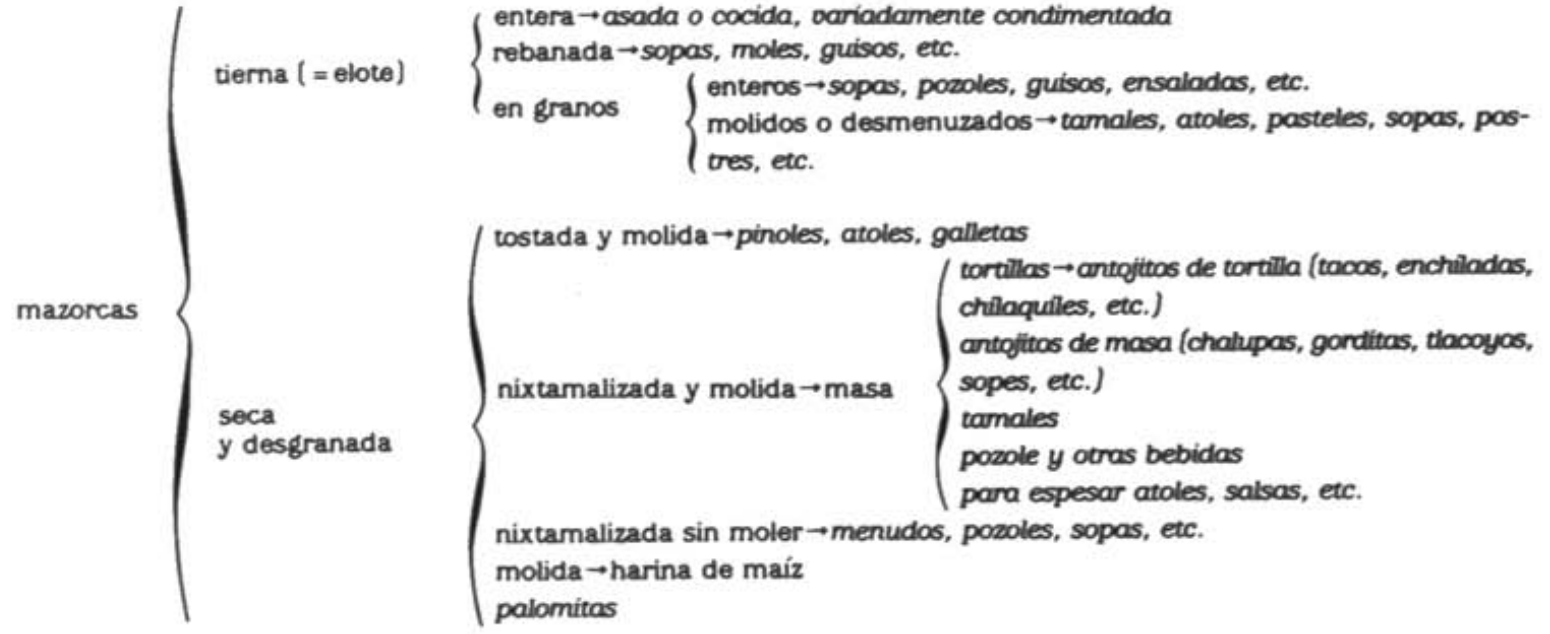
\includegraphics[width=\linewidth]{utilizaciondemaiz.png}
    \caption{
        \emph{Utilizacion del Maiz} (Maize Utilization) \cite{granlibro1988}.
    }
    \label{structures}
\end{figure}
 However, an ethical problem arises when it comes to showing this information to non-Spanish-speaking users because this book (and others) can only be found in Spanish. To show things like the diagram or other important information, I would first have to translate it and that can bring about translation misrepresentation. An article about cultural misrepresentation through translations first brings up the importance of literature in relation to culture. It says, “Literature represents a body of cultural goods that a particular culture sees as its heritage for its own members (self) and as an image for export to members of other cultures (other)” \cite{translationmisrep2008}. This is exceptionally important for this project because I will try to take the information and cultural representation from these texts written in Spanish and translate them in a manner that accurately reflects what Mexican culture is and there is the possibility of flaws coming along with that. In the article, they also bring up how the basic error of the translator is that they try to mold the meaning of the language being translated into one that fits the language it is being translated to \cite{translationmisrep2008}. This could have a negative impact on the project because in an effort to make a reading make sense in English, I could change the meaning it had in Spanish. In addition to that, there are words in Spanish that aren’t translatable to English and I would therefore be molding the meaning to what I think it means. This would make my project unethical in the sense that I could be mistranslating or changing the meaning of things from the original to my project.  


\section{Implicit Bias}
Finally, one of the largest possibilities for ethical concerns in this project is my own implicit bias as the curator of this project. Although I am Mexican and have grown up surrounded by Mexican culture I am in no way an all-knowing person when it comes to what is Mexican and what isn’t. Therefore, when creating the storyline for this project and assessing what should and shouldn’t be included, there is the risk of my implicit bias affecting the impression of what people learn about Mexican culture after using the experience. Implicit bias is an important ethical issue to consider because it is an unconscious way a person can be biased towards something. An article about the subject described how teachers can show bias towards students when it came to making a judgment call on disciplinary actions that have more subjective parameters such as what it means to be ‘disrespectful’ or ‘disruptive’ \cite{implicitbias201516}. They found that the students of color were more likely to be disciplined because of the teachers’ experience and unconscious associations with race \cite{implicitbias201516}. This is relevant to my project because it shows that people's biases can come out when making decisions on subjective matters even if they are not consciously aware of it. This could be reflected in the recipes that I choose for the experience. I have grown up and enjoyed the food made by my parents who are from the Mexican states of Zacatecas and Morelos. Therefore, I will be less likely to choose a dish more traditional to the state of Chiapas because I either have not tried it or it is just not part of what I consider to be good food. While these are examples I can point out, the whole idea behind implicit bias is that I won't know I am being biased towards something. At the end of the day, this project can be unethical in the sense that I will still be making the final judgment calls on what will go into the project and therefore my bias will affect the story told to favor my experience as a Mexican person. 

\section{Conclusion}
Overall, the purpose of this VR project is to teach and challenge people’s view of what Mexican culture is further than just tacos and tequila. This will be accomplished through a farm-to-table VR experience that allows people to experience Mexican food preparation short of actually making it themselves. However, this does not mean the project itself will be ethical. Using VR as a platform means that the project won’t be accessible to all because of the limited number of VR headset owners, and even those who do have access still run the risk of motion sickness. The initial version of this project will also be unethical in that it won’t be able to meet the accessibility needs of people with impaired movement because of my limited time and experience with this topic. When it comes to the content of this project, there are risks of the translations misrepresenting what the original Spanish-written text means in favor of making sense in English. In addition, the content can be biased during the curation process in favor of what I have experienced in Mexican culture. Finally, there is the question of whether this is the appropriate solution to teach and change people’s points of view toward Mexican culture. Perhaps a more hands-on approach would be a better and more in-depth learning experience than a 'quick and easy' technological solution. All of these are good points to make and even with my best efforts to avoid these faults, there will be ethical issues with this project. 


\printbibliography 

\end{document}
